\documentclass[%
 reprint,
%superscriptaddress,
%groupedaddress,
%unsortedaddress,
%runinaddress,
%frontmatterverbose, 
%preprint,
%preprintnumbers,
%nofootinbib,
%nobibnotes,
%bibnotes,
 amsmath,amssymb,
 aps,
%pra,
%prb,
%rmp,
%prstab,
%prstper,
%floatfix,
]{revtex4-2}
\usepackage{multirow}
\usepackage{graphicx}% Include figure files
\usepackage{dcolumn}% Align table columns on decimal point
\usepackage{bm}% bold math
%\usepackage{hyperref}% add hypertext capabilities
%\usepackage[mathlines]{lineno}% Enable numbering of text and display math
%\linenumbers\relax % Commence numbering lines

%\usepackage[showframe,%Uncomment any one of the following lines to test 
%%scale=0.7, marginratio={1:1, 2:3}, ignoreall,% default settings
%%text={7in,10in},centering,
%%margin=1.5in,
%%total={6.5in,8.75in}, top=1.2in, left=0.9in, includefoot,
%%height=10in,a5paper,hmargin={3cm,0.8in},
%]{geometry}
\usepackage[utf8x]{inputenc} % Включаем поддержку UTF8  
\usepackage[russian]{babel}  % Включаем пакет для поддержки русского языка 
\usepackage[normalem]{ulem}  % для зачекивания текста

\usepackage[noend]{algorithmic}
\def\algorithmicrequire{\textbf{Вход:}}
\def\algorithmicensure{\textbf{Выход:}}
\def\algorithmicif{\textbf{если}}
\def\algorithmicthen{\textbf{то}}
\def\algorithmicelse{\textbf{иначе}}
\def\algorithmicelsif{\textbf{иначе если}}
\def\algorithmicfor{\textbf{для}}
\def\algorithmicforall{\textbf{для всех}}
\def\algorithmicdo{}
\def\algorithmicwhile{\textbf{пока}}
\def\algorithmicrepeat{\textbf{повторять}}
\def\algorithmicuntil{\textbf{пока}}
\def\algorithmicloop{\textbf{цикл}}
% переопределение стиля комментариев
\def\algorithmiccomment#1{\quad// {\sl #1}}

\usepackage{caption}
\usepackage{subcaption}
\usepackage{multirow}
\usepackage[table,xcdraw]{xcolor}
\begin{document}



\title{Лабораторная работа 8.1\\Тепловое излучение}% Force line breaks with \\



\author{Батарин Егор Владиславович}
\affiliation{%
 Студент 3 курса РТ\\
}%

\collaboration{Московский физико-технический институт}%\noaffiliation

\date{6 октября 2021 г.}% It is always \today, today,
             %  but any date may be explicitly specified
             

\begin{abstract}
При помощи модели АЧТ проводятся измерения температуры оптическим пирометром с исчезающей нитью и термопарой, исследуются излучение накаленных тел с различной испускательной способностью, определяются постоянные Планка и Стефана-Больцмана.
\begin{description}
\item[Оборудование]
Пирометр, неоновая лампочка, модель АЧТ, разогретые кольца.
\end{description}
\end{abstract}

%\keywords{Suggested keywords}%Use showkeys class option if keyword
                              %display desired
\maketitle

%\tableofcontents

\section{Теоретическая часть.}

В работе производится измерение яркостной температуры тела при помощи оптического спектрометра. Нить считается откалиброванной на теле, если она "исчезает" на нем. В этом случае можно измерить яркостную температуру тела. Если тело не абсолютно черное, то эта температура будет ниже термодинамической, так как нечерное тело излучает меньше, чем АЧТ. 


\section{Экспериментальная установка и методика}

В работе проверяется закон Стефана-Больцмана для нити (предполагается, что она излучает как серое тело):
$$W  = \varepsilon_T S \sigma T^4$$
Для этого предполагается, что $W = \varepsilon_T B T^n$, что равносильно наличию линейной зависимости $\ln W = \ln(\varepsilon_T B) + n\ln T$, которая проверяется по МНК.

Ясно, что $B = S\sigma$, причем $S = 0,36 \text{ см}^2$. Постоянная Стефана-Больцмана равна $\sigma = \frac{W}{\varepsilon_T S T^4}$, ее измеряем для температур, больших 1700 К. После этого вычисляем постоянную Планка $h = \sqrt[3]{\frac{2\pi^5k^4}{15c^2\sigma}}$.

\section{Основные результаты и их обсуждение}

Потенциированная зависимость Стефана-Больцмана имеет вид:
\begin{figure}[h]
	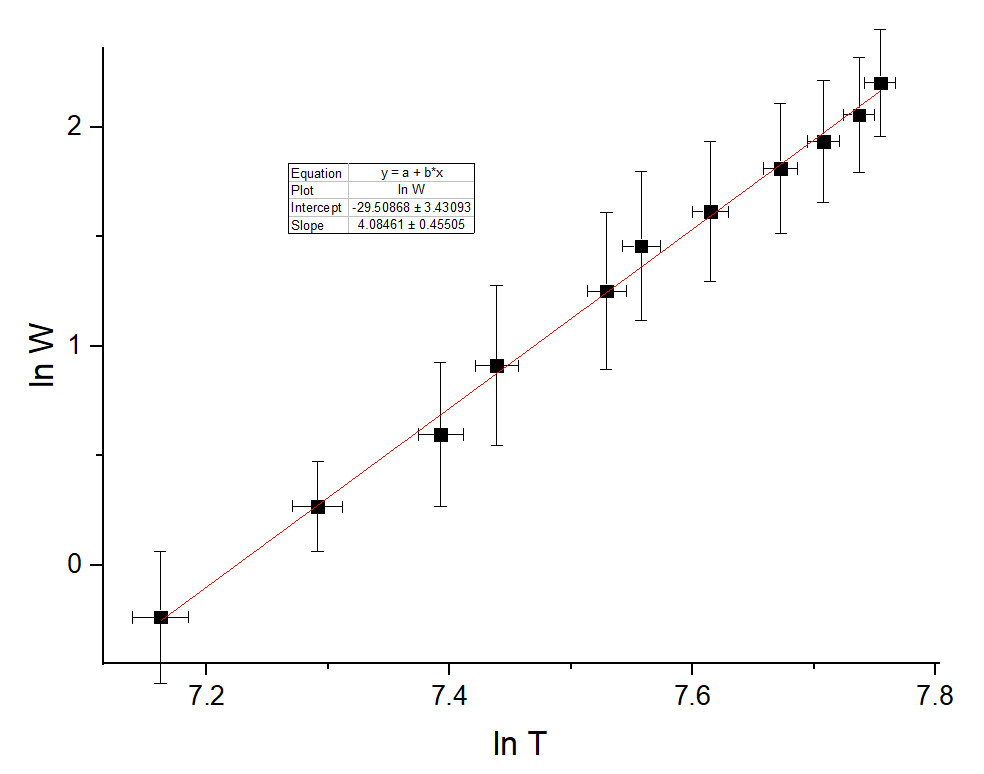
\includegraphics[scale=0.8]{1.png}
\end{figure}

Из обобщенного МНК следует, что $n = 4 \pm 0.5$, что соответствует теории. Все остальные измеренные и помереные величины сведены в таблицу:

\begin{table}[]
	\begin{tabular}{lll|l|l|l|l|l|lll}
		\hline
		\multicolumn{1}{|l|}{Яркость, К} & \multicolumn{1}{l|}{Вольт} & Ампер & $W$, Вт        & $D(W)$            & $\ln W$              & $D(\ln W)$    & $T$,К           & \multicolumn{1}{l|}{$D(T)$, К} & \multicolumn{1}{l|}{$\ln T$}  & \multicolumn{1}{l|}{$D(\ln T)$} \\ \hline
		\multicolumn{1}{|l|}{1245}       & \multicolumn{1}{l|}{1.678} & 0.47  & 0.78866        & 0.015773          & -0.23742             & 0.301042     & 1289.5          & \multicolumn{1}{l|}{30}        & \multicolumn{1}{l|}{7.16201}  & \multicolumn{1}{l|}{0.023265}   \\ \hline
		\multicolumn{1}{|l|}{1407}       & \multicolumn{1}{l|}{2.38}  & 0.55  & 1.309          & 0.02618           & 0.269263             & 0.205702     & 1467.7          & \multicolumn{1}{l|}{30}        & \multicolumn{1}{l|}{7.291452} & \multicolumn{1}{l|}{0.02044}    \\ \hline
		\multicolumn{1}{|l|}{1549}       & \multicolumn{1}{l|}{2.98}  & 0.61  & 1.8178         & 0.036356          & 0.597627             & 0.328764     & 1623.9          & \multicolumn{1}{l|}{30}        & \multicolumn{1}{l|}{7.392586} & \multicolumn{1}{l|}{0.018474}   \\ \hline
		\multicolumn{1}{|l|}{1619}       & \multicolumn{1}{l|}{3.66}  & 0.68  & 2.4888         & 0.049776          & 0.911801             & 0.366362     & 1700.9          & \multicolumn{1}{l|}{30}        & \multicolumn{1}{l|}{7.438913} & \multicolumn{1}{l|}{0.017638}   \\ \hline
		\multicolumn{1}{|l|}{1765}       & \multicolumn{1}{l|}{4.6}   & 0.76  & 3.496          & 0.06992           & 1.251619             & 0.358015     & 1861.5          & \multicolumn{1}{l|}{30}        & \multicolumn{1}{l|}{7.529138} & \multicolumn{1}{l|}{0.016116}   \\ \hline
		\multicolumn{1}{|l|}{1814}       & \multicolumn{1}{l|}{5.3}   & 0.81  & 4.293          & 0.08586           & 1.456986             & 0.339386     & 1915.4          & \multicolumn{1}{l|}{30}        & \multicolumn{1}{l|}{7.557682} & \multicolumn{1}{l|}{0.015663}   \\ \hline
		\multicolumn{1}{|l|}{1916}       & \multicolumn{1}{l|}{5.85}  & 0.86  & 5.031          & 0.10062           & 1.615619             & 0.321133     & 2027.6          & \multicolumn{1}{l|}{30}        & \multicolumn{1}{l|}{7.614608} & \multicolumn{1}{l|}{0.014796}   \\ \hline
		\multicolumn{1}{|l|}{2026}       & \multicolumn{1}{l|}{6.66}  & 0.92  & 6.1272         & 0.122544          & 1.812738             & 0.295851     & 2148.6          & \multicolumn{1}{l|}{30}        & \multicolumn{1}{l|}{7.672572} & \multicolumn{1}{l|}{0.013963}   \\ \hline
		\multicolumn{1}{|l|}{2096}       & \multicolumn{1}{l|}{7.22}  & 0.96  & 6.9312         & 0.138624          & 1.936033             & 0.279321     & 2225.6          & \multicolumn{1}{l|}{30}        & \multicolumn{1}{l|}{7.707782} & \multicolumn{1}{l|}{0.01348}    \\ \hline
		\multicolumn{1}{|l|}{2156}       & \multicolumn{1}{l|}{7.82}  & 1     & 7.82           & 0.1564            & 2.056685             & 0.263003     & 2291.6          & \multicolumn{1}{l|}{30}        & \multicolumn{1}{l|}{7.737006} & \multicolumn{1}{l|}{0.013091}   \\ \hline
		\multicolumn{1}{|l|}{2193}       & \multicolumn{1}{l|}{8.62}  & 1.05  & 9.051          & 0.18102           & 2.202875             & 0.243385     & 2332.3          & \multicolumn{1}{l|}{30}        & \multicolumn{1}{l|}{7.75461}  & \multicolumn{1}{l|}{0.012863}   \\ \hline
		&                            &       & \textbf{$T$,К} & \textbf{$\sigma$} & \textbf{$D(\sigma)$} & \textbf{$h$} & \textbf{$D(h)$} &                                &                               &                                 \\ \cline{4-8}
		&                            &       & 1700.9         & 3.93E-08          & 7.87E-10             & 6.9E-34      & 1.84E-35        &                                &                               &                                 \\ \cline{4-8}
		&                            &       & 1861.5         & 3.52E-08          & 7.03E-10             & 7.17E-34     & 1.91E-35        &                                &                               &                                 \\ \cline{4-8}
		&                            &       & 1915.4         & 3.69E-08          & 7.38E-10             & 7.05E-34     & 1.88E-35        &                                &                               &                                 \\ \cline{4-8}
		&                            &       & 2027.6         & 3.67E-09          & 7.35E-11             & 1.52E-33     & 4.06E-35        &                                &                               &                                 \\ \cline{4-8}
	\end{tabular}
\end{table}


\section{Заключение}

Была проверена степенная зависимость Стефана-Больцмана, она оказалась в эксперименте такой, как в теории. Получены близкие к теоретическим значения постоянной Планка и Стефана-Больцмана.
\end{document}